\documentclass[12pt,preprint]{aastex}
% for \sout
\usepackage{ulem}
% makes sure \em{} is italic rather than underlined (corrects ulem from line above)
\normalem

% for the red MarginPars
\usepackage{color}

% some extra math symbols
\usepackage{mathtools}

% allows Greek symbols to be bold
\usepackage{bm}

\newcommand{\rhocutoff}{\rho_\mathrm{cutoff}}
\newcommand{\rhoanelastic}{\rho_\mathrm{anelastic}}

\newcommand{\gcc}{\mathrm{g~cm^{-3} }}
\newcommand{\Tcutoff}{T_\mathrm{cutoff}}

% MarginPars
\setlength{\marginparwidth}{0.75in}
\newcommand{\MarginPar}[1]{\marginpar{\vskip-\baselineskip\raggedright\tiny\sffamily\hrule\smallskip{\color{red}#1}\par\smallskip\hrule}}


\newcommand{\evm}{{(-)}}
\newcommand{\evz}{{(\circ)}}
\newcommand{\evp}{{(+)}}
\newcommand{\enu}{{(\nu)}}



\newcommand{\msolar}{\mathrm{M}_\odot}

\begin{document}

%==========================================================================
% Title
%==========================================================================
\title{Double White Dwarf Mergers with CASTRO\\ I. Methodology and Code 
       Verification}

\shorttitle{DWD Mergers. I. Methodology}
\shortauthors{Max}

\author{TBD}
%==========================================================================
% Abstract
%==========================================================================
\begin{abstract}
We describe our numerical methodology for modeling double white dwarf
systems with the AMR hydrodynamics code Castro.

\end{abstract}
\keywords{hydrodynamics - methods: numerical - supernovae: general - white dwarfs}

%==========================================================================
% Introduction
%==========================================================================
\section{Introduction}

Type Ia supernovae (SNe Ia) are currently some of the most exciting events to study in astrophysics. These bright, brief pulses of light in the distant universe have led to a number of important discoveries in recent years, including the discovery of the accelerated expansion of the universe \citep{perlmutter1999,riess1998}. However, their origin is shrouded in mystery. It has long been expected that these events arise from the thermonuclear explosions of white dwarfs \citep{hoyle_fowler:1960}, but the cause of these explosions is uncertain. In particular, it is not clear what process causes the temperatures in these white dwarfs to become hot enough for explosive burning of its constituent nuclei. The model favored initially by the community was the so-called single-degenerate (SD) model \citep{whelan_iben:1973}. Accretion of material from a companion star such as a red giant would cause the star to approach the Chandrasekhar mass, and in doing so the temperature and density in the center would become sufficient for thermonuclear fusion to proceed. However, in recent years many alternative progenitor models have been discussed. A leading candidate for explaining some or most of these explosions is the double-degenerate model, in which two white dwarfs merge and the merged object reaches the conditions necessary for a thermonuclear ignition \citep{ibentutukov:1984,webbink:1984}. Another is the double detonation scenario, where accretion of material onto a sub-Chandrasekhar white dwarf would lead to a detonation inside the accreted envelope, and this would send a compressional wave into the core of the star that would trigger a secondary detonation. A recent review of the progenitor models can be found in \citet{hillebrandt:2013}.

There are several observational reasons why double-degenerate systems are a promising progenitor system for at least a substantial fraction of normal SNe Ia. No conclusive evidence exists for a surviving companion star of a SN Ia; this is naturally explained by the DD model because both WDs are destroyed in the merger process. Similarly, pre-explosion images of the SN Ia systems have never clearly turned up a companion star, and in some cases a large fraction of the SD parameter space is excluded. Additionally, not enough progenitor systems are seen for the SD case to match the observed local SN Ia rate, whereas the number of white dwarf binaries may be sufficient to account for this rate. Finally, the DD model can naturally explain the fact that many SNe Ia are observed to occur at very long delay times after the stars were formed, since the progenitor systems only become active once both stars have evolved off the main sequence. A thorough review of the observational evidence about SNe Ia and further discussion of these ideas can be found in \cite{maoz:2014}.  

The history of double degenerate theory can broadly be described as a series of three major paradigm shifts. The first attempts to model the results of the merger process came in the 1980s. \cite{nomotoiben:1985} demonstrated that if the secondary overflowed its Roche lobe and its mass accreted onto the primary near the Eddington rate, that off-center carbon ignition would occur. \cite{saionomoto:1985} tracked the evolution of the flame and found that it propagated quiescently into the center, converting the carbon-oxygen white dwarf into an oxygen-neon-magnesium white dwarf. This would then be followed by collapse into a neutron star -- a result with significantly different observational properties compared to a SN Ia. This scenario, termed accretion-induced collapse, would be avoided only if the accretion rate were well below the Eddington rate. \cite{tutukov_yungelson:1979} observed that this could happen if the mass loss from the secondary was higher than the Eddington rate and thus the accreted material formed an accretion disc, which might rain down on the primary more slowly. The main finding was that double degenerate systems would not obviously lead to Type Ia supernovae.

The first three-dimensional simulations of double degenerate systems were performed by \citet{benz:1990}, who used the smoothed particle hydrodynamics (SPH) method to simulate the merger process. They found that if the lower-mass secondary was close enough to the primary to begin mass transfer on a dynamical time scale, the secondary completely disrupted and formed a hot envelope on the primary, with a centrifugally-supported accretion disk surrounding the core and envelope. They noted that the envelope temperature was hot enough to generate carbon fusion but neglected reactions in their simulation. Later simulations of similar setups \citep{rasio_shapiro:1995,yoon:2007,loren-aguilar:2009,raskin:2012} corroborated this result. This validation of the prediction of \cite{tutukov_yungelson:1979} did not instill confidence in the community. \cite{mochkovitch_livio:1990} and \cite{livio:2000} observed that turbulent viscosity would be sufficiently large for angular momentum to be removed from the disk at a rate high enough to generate these troublesome accretion timescales. Based on all of this evidence, the review of \cite{hillebrandtniemeyer2000} argued that the model was only viable if the accretion-induced collapse problem could be avoided. Later work by \cite{shen:2012} and \cite{schwab:2012} used a more detailed treatment of the viscous transport in the outer regions of the remnant and found that while the centrifugally supported envelope would be converted into hot envelope material on a viscous timescale, their simulations still led to off-center carbon burning. \cite{vankerkwijk:2010} argued that equal-mass mergers would lead to the conditions necessary for carbon detonation in the center of the merged object, but \cite{shen:2012} questioned this for similar reasons related to how viscous transport would convert rotational motion into pressure support. \cite{zhu:2013} followed this with an expanded parameter space study and argued that many of their carbon-oxygen systems had the potential to detonate. The study of the long-term evolution of the remnants is thus still an open subject of research.

The most recent shift in perspective on this problem started with two series of papers appearing at roughly the same time. One began with \cite{pakmor:2010} and \cite{pakmor:2011}. This group used the SPH method to study the merger of equal-mass ($0.9\ M_\odot$) carbon-oxygen white dwarfs and found that a hotspot was generated near the surface of the primary white dwarf. They argued that this region had a temperature and density sufficient to trigger a thermonuclear detonation. They propagated this detonation throughout the system and found that it would observationally appear as a subluminous Type Ia supernova. This was the first time any simulation successfully reproduced at least some characteristics of a SN Ia. \cite{pakmor:2011} tried a few different mass combinations and found empirically that this would hold as long as the secondary was at least 80\% as massive as the primary. These events, where the merger process resulted in the detonation of the system during the merger coalescence -- avoiding the much longer time-scale evolution -- were termed ``violent'' mergers.

Around the same time, however, \cite{guillochon:2010} and \cite{dan:2011} came to significantly different conclusions. They pointed out that the previously mentioned simulations generally all shared a significant drawback, which was that their initial conditions were not carefully constructed. \cite{motl:2002}, \cite{dsouza:2006}, and \cite{motl:2007} (the first three-dimensional grid-based simulations of white dwarf mergers) pioneered the study of looking at the long-term dynamical evolution of merger scenarios after constructing exact equilibrium initial conditions. In contrast to the other studies, they found that paying close attention to the accuracy of the initial conditions of the simulation has important effects. In particular, earlier work placed the stars too close together and ignored the effects of tidal forces on changing the shape of the secondary, leading to the merger happening artificially too quickly. When the initial conditions are constructed in exact equilibrium, the system can be stable for tens of orbital periods, substantially changing the character of the mass transfer phase. However, one limitation of this work is that the authors used a polytropic equation of state and thus could not consider nuclear reactions. \cite{guillochon:2010} and \cite{dan:2011} improved on this using a realistic equation of state, a nuclear reaction network, and a similar approach to the equilibrium initial conditions, and found substantial agreement with the idea that mass transfer occurs in a stable manner over tens of orbital periods. They also found that, assuming the material accreted onto the surface of the primary was primarily helium, explosive surface detonations would occur as a result of accretion stream instabilities during the mass transfer phase prior to the full merger. This could trigger a double-detonation explosion and thus perhaps a SN Ia.

The most recent developments give some areas of agreement and some of remaining uncertainty. \cite{pakmor:2012} performed a merger scenario with a $1.1\ M_\odot$ and $0.9\ M_\odot$ setup, with better treatment of the initial conditions, and also found that the merger process happened over more than ten orbits. Nevertheless, they still found that a carbon-oxygen detonation would occur, in line with their earlier results. \cite{moll:2014} was also able to find a detonation in a similarly massive system. \cite{dan:2012} and \cite{dan:2014} performed a large sweep of the parameter space for merger pairs and found that pure carbon-oxygen systems would generally not lead to detonations and violent mergers except for the most massive systems. They did find that for systems containing helium, many of them would detonate and potentially lead to SNe Ia, either through the aforementioned instabilities in the accretion stream, or during the contact phase, similar to the violent carbon-oxygen mergers. \cite{pakmor:2013} added a thin helium shell on their primary white dwarf, and found that this robustly led to a detonation of the white dwarf. Thus at least a preliminary agreement may be that systems containing helium could robustly lead to events resembling SNe Ia, as well as very massive carbon-oxygen binaries. 

This is the first in a series of papers designed to address these outstanding theoretical issues for white dwarf mergers. This work will discuss the verification of our hydrodynamics code for simulating these events. Later efforts will look at the initial conditions of the system, the robustness with which a hotspot is found from which a detonation could occur, and the importance of the initial white dwarf models, which should be more sophisticated than simple carbon-oxygen mixtures and in principle should use results from modern stellar evolution calculations. Section \ref{sec:Numerical Methodology} describes our code and why it can provide useful results compared to other methodologies used for this problem. Section \ref{sec:Tests} discusses a few test problems that we use to demonstrate that our code accurately solves the equations of fluid dynamics. Section \ref{sec:Performance} demonstrates that the software scales well for supercomputer applications. Finally, Section \ref{sec:Conclusions and Discussion} recaps what we have shown and highlights some of the future work we plan to do.

%==========================================================================
% Numerical Methodology
%==========================================================================
\section{Numerical Methodology}\label{sec:Numerical Methodology}

\subsection{Hydrodynamics}

To study the white dwarf merger problem, we use the grid-based hydrodynamics code CASTRO \citep{castro}. CASTRO solves the Euler equations, along with the inclusion of optional modules for gravity, nuclear reactions and thermodynamics. We direct the reader to the original code paper for a description of CASTRO's approach to solving the equations of hydrodynamics. In this work, we report only on the changes we have made to the code since its original release, for the purpose of approaching this problem. CASTRO is based on the BoxLib adaptive-mesh refinement (AMR) framework (ref), which represents fluid data on a mesh where regions of interest have higher spatial resolution. CASTRO is highly parallel and is designed for large-scale use on modern supercomputers; see Section \ref{sec:Performance} for information on how CASTRO performs for our problem.

We use the unsplit piecewise-parabolic method (PPM) solver in CASTRO to advance the hydrodynamics system in time \citep{ppmunsplit}.  A number of changes were made to the solver, which are detailed in the Appendix.  These changes bring the algorithm more in line with that of \cite{ppm}. CASTRO as originally released featured a slightly modified version of the higher resolution limiters of \cite{colella_sekora:2008}, which can be accessed in the code using \texttt{castro.ppm\_type = 2}. The advantage of this limiter is that it preserves physical extrema rather than clipping them off as in the original approach of \cite{ppm}. However, we found these limiters to be unsatisfactory for our problem. There are many regions in our problem with large density gradients (such as the interface between the star's atmosphere and the ambient gas outside of it) and in these regions the algorithm can yield negative densities. This often results from the limiters interpreting these gradients as being true minima. As a result, we use the original limiter, which is strictly monotonicity preserving in the parabolic profiles it generates; this is activated with \texttt{castro.ppm\_type = 1}.

A related issue that required a code improvement was that in cases of large density gradients such as the edge of a star, it is possible to generate negative densities in zones even with the more strongly limited PPM. This can occur if a region of large density is moving away from an ambient zone at relatively large speeds; then the net density flux in the ambient zones can be large enough to unphysically drag the density below zero. In practice, this will occur at the trailing edge of a star that is moving across a grid. In such a situation, there are two main approaches one could take: either explicitly introduce a positivity-guaranteeing diffusive flux, or reset the characteristics of the affected zone. We choose the latter approach. Even though it is non-conservative, it preserves a characteristic we value, which is to keep the edge of the stars relatively sharp, as they physically should be. Since the mass of the affected zones is typically already fairly low, this should not seriously affect the energy conservation properties of our simulation. Similarly, it is also possible in this physical situation for very large velocities to be generated in the material behind the star. The momentum transferred to the ambient zone is close to the momentum of the stellar material, but this is of much higher density and so the velocity of the ambient material must become very large to compensate. While this may be physically viable in certain circumstances, it poses a problem for our code, which uses subcycling in time (see below). The timestep is fixed at the beginning of the set of subcycled timesteps, and if in the middle of the cycle a velocity is generated that is so large that it violates the CFL criterion for this timestep, we cannot guarantee the stability of the resulting solution since we cannot alter the timestep. (Nor would we want to, because in some cases because the velocity becomes spuriously large and would drag down the global timestep.) Therefore we also insert a check at the end of every hydrodynamics timestep that resets the velocity and/or sound-speed (indirectly, using the temperature) of any zone that violates the CFL criterion given the timestep we chose at the beginning of the cycle. In practice, we find that this is mainly necessary only for simulations in the inertial reference frame of the white dwarf merger, which we do not normally do for the reasons stated in Section \ref{Sec:Kepler}.

The boundary conditions on the hyperbolic system are simply zero-gradient zones that allow material to flow directly out of the domain. Using AMR, we make the coarse grid very large, so as
to place the boundaries far from the region of interest. This ensures that any boundary effects do not pollute the inner region where the stars will eventually make contact.  We further
make the restriction that only level-0 (coarse) grids can touch the domain boundary.

CASTRO's approach to adaptive mesh refinement, based on its underlying BoxLib framework, is to refine zones based on certain user-specified criteria that tag regions of interest for higher spatial resolution. Data is represented on one of a number of AMR levels, where each level corresponds to a set of zones at the same resolution, which covers a subset of the domain covered by the level immediately below it. We typically call the level 0 grid the \textit{coarse} grid, which has the lowest spatial resolution. Each finer, higher-level grid has a higher resolution than the grid below it by some integer factor $N$, which is restricted to be $N = 2\ \text{or}\ 4$ in the code. The zones are strictly contained within the rectangular extent of the underlying coarser zones (the code is not restricted to representing only Cartesian geometries, but we use a Cartesian mesh with uniform spacing in each dimension for the present study). For the time evolution of the AMR system we use subcycling, where each AMR level is advanced at a different timestep and a correction step is applied at the end to synchronize the various levels. Generally the number of subcycled timesteps is equal to the jump in refinement between levels, so for example on a grid with three levels and two jumps of four in refinement, the level 2 zones will have 16 times higher spatial resolution than the coarse grid and there will be 16 level 2 timesteps per level 0 timestep.

For the evolution of binary systems, it is most natural to evolve the two stars in a frame that is co-rotating at the same period as the orbital period. CASTRO has the ability to evolve systems in a rotating reference frame, as discussed in the original code paper. Source terms corresponding to the Coriolis and centrifugal force terms are added to the momentum and energy equations. In this frame, the stars essentially remain stationary in their original positions due to the centrifugal force supporting against the gravitational attraction, and will remain this way as long as significant mass transfer does not occur. \cite{swesty00} demonstrated (in the context of neutron star mergers) that conservation of angular momentum is much easier to obtain in the rotating reference frame than in an inertial frame in which stars advect large amounts of material around the domain. We wish to emphasize that although it is commonly stated in the literature that grid-based codes poorly conserve angular momentum, this is not generally true. When the resolution is sufficiently high and a rotating reference frame is employed, excellent conservation properties can result, as demonstrated in Section \ref{Sec:Kepler}. We note that as the stars begin to coalesce, the rotating reference frame will no longer provide a good approximation to the spatial motion of the stars and then they will begin to significantly move around the domain. This is not necessarily problematic because the most important feature of the rotating frame is that it helps ensure that the initial coalescence is not the result of spurious numerical loss of angular momentum. When significant mass transfer sets in and evolution proceeds on a dynamical timescale, the conservation properties may be slightly worse but angular momentum conservation is also less important.

\subsection{Microphysics}

The equation of state (EOS) for our simulations is the Helmholtz EOS \citep{timmes_swesty:2000}. This models an electron-positron gas of arbitrary relativity and degeneracy over a wide range of temperatures and densities. Thermodynamic quantities are calculated as derivatives of the Helmholtz free energy, and the values are interpolated from a table. The natural variables of the Helmholtz free energy are temperature and density, and calling the EOS is simplest in this form. However, in hydrodynamics we often have the density, and internal energy as independent variables, and we want to obtain the temperature, pressure, and other quantities. To do this, we employ a Newton-Raphson iteration over the temperature (given some sufficient starting guess) until we find the temperature that corresponds to the desired internal energy. Sometimes this process fails to converge and the iterative value approaches zero. In these cases we employ a ``floor'' that limits how low the temperature can go (typically $10^4$ or $10^5$ K). There is a choice here how to proceed: we can either assign this floor value to the temperature and let that zone be thermodynamically inconsistent (the original behavior in Castro), or we can adjust the internal energy to be thermodynamically consistent with the temperature, at the cost of violating energy conservation. We have found in test problems of one-dimensional shocks that the latter yields more accurate results, so we employ the latter method.

Reactions?

\subsection{Initial Models}
\label{sec:initial_models}

We generate initial models by integrating the equation of hydrostatic
equilibrium, taking the temperature and composition to be constant,
and using the general stellar equation of state.  This results in
a single nonlinear equation to find the density in a zone given the
conditions in the zone beneath it:
\begin{equation}
\frac{p(\rho_{i+1}) - p_i}{\Delta x} = \frac{1}{2} (\rho_i + \rho_{i+1}) g_{i+1/2}
\end{equation}
This is solved via Newton iteration to give $\rho_{i+1}$.  Here, $g_{i+1/2}$
is the gravitational acceleration at the interface between zones $i$ and $i+1$,
found by simply adding up all the mass from zones $1, \ldots, i$ to get the
enclosed mass, $M_{i+1/2}$, and then $g_{i+1/2} = -GM_{i+1/2}/r_{i+1/2}^2$.

To start the integration off, we need a central density.  We guess at
this, and then iterate over the entire integration procedure to find
the central density needed to yield the desired total mass.  Finally,
we generate the initial model at the same resolution as the finest
grid in our simulation.

We map the 1-d model onto the 3-d Cartesian grid by taking density,
temperature, and composition as the independent variables,
interpolating these to the cell-centers, and then calling the equation
of state to initialize the remaining terms.  The velocity is taken to
be zero in the rotating frame initially.

\subsection{Gravity}

We solve the Poisson equation for self-gravity for our problem,
\begin{equation}
  \nabla^2 \Phi(\mathbf{x}) = -4\pi G\, \rho(\mathbf{x}),
\end{equation}
where $\Phi$ is the gravitational potential, $G$ is the gravitational constant, and $\rho$ is the mass density. We note that the sign convention used in CASTRO is opposite to that commonly seen in the physics literature, so that $\Phi$ is positive everywhere. The solution of this equation in CASTRO is described in \cite{castro}, and consists of both level and composite solves, and a final synchronization at the end.

\subsubsection{Boundary Conditions}

Analytic solutions to the Poisson equation customarily assume that the potential vanishes at large distances from the region of non-zero density. However, on a finite computational domain it is usually not possible to have the edges of the domain be far enough away that the potential can be taken to be zero there. Solving the Poisson equation therefore requires knowledge of the values of the potential on the edges of the computational domain. In principle, they can be computed by doing a direct sum over the mass distribution inside the domain, where the mass in each zone is treated as a point source:
\begin{equation}
  \Phi_{\text{lmn}} = G\, \sum_{\text{i, j, k}} \frac{G \rho_{\text{ijk}}}{|\mathbf{x}_{\text{lmn}} - \mathbf{x}_{\text{ijk}}|}\, \Delta V_{\text{ijk}}.\label{direct_sum}
\end{equation}
Here (i, j, k) are the indices of cells inside the domain, and (l, m, n) are the indices of boundary locations. $\Delta V$ is the volume of the zone. We have implemented this as an option\footnote{It is controlled with the \texttt{gravity.direct\_sum\_bcs} input parameter.} in CASTRO. If there are $N$ zones per spatial dimension, then there are $6 N^2$ boundary zones, and each boundary zone requires a sum over $N^3$ zones, so the direct computation of the boundary conditions scales as $N^5$.  This method is expensive enough that it is not used for hydrodynamics simulations (though it is useful for comparison to approximate solutions).

In a typical simulation we place the boundaries of the domain far enough away from the region containing most of the mass that some method of approximation to this direct summation is justified. Many approaches exist in the literature. The original release of CASTRO featured the crudest possible approximation: a monopole prescription, where the boundary values were computed by summing up all the mass on the domain and treating it as a point source at the domain center. This is exactly correct only for a spherically symmetric mass distribution, and indeed this is often a sufficient approximation for single-star Type Ia supernova simulations that employ self-gravity (ref). However, for a problem like that of a binary star system with significant departures from spherical symmetry, this assumption fails to produce accurate boundary values. This results in a significant drift of the center of the mass of the system over time. 

The most natural extension of the monopole prescription is to include higher-order multipole moments. If the entire mass distribution is enclosed, then the potential can be expanded in a series of spherical harmonics $Y_{lm}$:
\begin{equation}
  \Phi(\mathbf{x}) = \sum_{l=0}^{\infty}\sum_{m=-l}^{l} \frac{4\pi}{2l + 1} q_{lm} \frac{Y_{lm}(\theta,\phi)}{r^{l+1}}, \label{spherical_harmonic_expansion}
\end{equation}
where $q_{lm}$ are the so-called multipole moments. The origin of the coordinate system is taken to be the center of the computational domain, and $r$ is the distance to the origin. The multipole moments can be calculated by expanding the Green's function for the Poisson equation as a series of spherical harmonics.
\begin{comment}
, which yields
\begin{equation}
  q_{lm} = \int Y^*_{lm}(\theta^\prime, \phi^\prime)\, {r^\prime}^l \rho(\mathbf{x}^\prime)\, d^3x^\prime. \label{multipole_moments_original}
\end{equation}
\end{comment}
After some algebraic simplification of Equation \ref{spherical_harmonic_expansion} using the addition theorem for spherical harmonics,
\begin{comment}
\begin{align}
  &\frac{4\pi}{2l+1} \sum_{m=-l}^{l} Y^*_{lm}(\theta^\prime,\phi^\prime)\, Y_{lm}(\theta, \phi) = P_l(\text{cos}\, \theta) P_l(\text{cos}\, \theta^\prime) \notag \\
  &\ \ + 2 \sum_{m=1}^{l} \frac{(l-m)!}{(l+m)!} P_{l}^{m}(\text{cos}\, \theta)\, P_{l}^{m}(\text{cos}\, \theta^\prime)\, \left[\text{cos}(m\phi)\, \text{cos}(m\phi^\prime) + \text{sin}(m\phi)\, \text{sin}(m\phi^\prime)\right].
\end{align}
\end{comment}
the potential outside of the mass distribution can be written as:
\begin{equation}
  \Phi(\mathbf{x}) = \sum_{l=0}^{\infty} \left[Q_l^{(0)} \frac{P_l(\text{cos}\, \theta)}{r^{l+1}} + \sum_{m = 1}^{l}\left[ Q_{lm}^{(C)}\, \text{cos}(m\phi) + Q_{lm}^{(S)}\, \text{sin}(m\phi)\right] \frac{P_{l}^{m}(\text{cos}\, \theta)}{r^{l+1}} \right].\label{multipole_potential}
\end{equation}
$P_l(x)$ are the Legendre polynomials and $P_{l}^{m}(x)$ are the associated Legendre polynomials. $Q_l^{(0)}$ and $Q_{lm}^{(C,S)}$ are variants of the multipole moments that involve integrals of $P_l$ and $P_l^m$, respectively, over the computational domain.
\begin{comment}
\begin{align}
  Q_l^{(0)}   &= \int P_l(\text{cos}\, \theta^\prime)\, {r^{\prime}}^l \rho(\mathbf{x}^\prime)\, d^3 x^\prime \\
  Q_{lm}^{(C)} &= 2\frac{(l-m)!}{(l+m)!} \int P_{l}^{m}(\text{cos}\, \theta^\prime)\, \text{cos}(m\phi^\prime)\, {r^\prime}^l \rho(\mathbf{x}^\prime)\, d^3 x^\prime \\
  Q_{lm}^{(S)} &= 2\frac{(l-m)!}{(l+m)!} \int P_{l}^{m}(\text{cos}\, \theta^\prime)\, \text{sin}(m\phi^\prime)\, {r^\prime}^l \rho(\mathbf{x}^\prime)\, d^3 x^\prime.
\end{align}
\end{comment}
This approach becomes computationally feasible when we cut off the outer summation in Equation \ref{multipole_potential} at some finite value of $l_{\text{max}}$. If it is of sufficiently high order, we will accurately capture the distribution of mass on the grid. In practice we first evaluate the discretized analog of the modified multipole moments for $0 \leq l \leq l_{\text{max}}$ and $1 \leq m \leq l$, an operation that scales as $N^3$. We then directly compute the value of the potential on all of the $6N^2$ boundary zones. Since the multipole moments only need to be calculated once, the full operation scales only as $N^3$. The amount of time required to calculate the boundary conditions will be directly related to the chosen value of $l_{\text{max}}$, so there is a trade-off between computational expense and accuracy of the result. We find that for the early stages of the evolution of the binary system, $l_\text{max} \approx 6$ is sufficient.

%==========================================================================
% Test Problems
%==========================================================================
\section{Test Problems}\label{sec:Tests}

In this section we describe a series of test problems that couple the hydrodynamics, gravity, and EOS modules.

\subsection{Maintaining Hydrostatic Equilibrium}\label{Sec:HSE}

In Section \ref{sec:initial_models} we describe the process by which we generate initial stellar models. While the 1D models are in hydrostatic equilibrium to within a small error, interpolation onto the 3D Cartesian grid will introduce perturbations into the solution \citep{zingale:2002}. Although we ensure that the initial models are generated with the same equation of state and are as well resolved as our finest grid, there will still be a hydrodynamical error associated with the fact that the rectangular grid cannot faithfully represent a spherical star. Additionally, the gravitational potential obtained by the multigrid solver will differ slightly from the one assumed by the initial model, and the operator splitting between the gravity and hydrodynamics should also result in small errors. As a result, we expect that the star will oscillate slightly about an equilibrium point, but that the amplitude of this oscillation should decrease with increasing resolution.

\subsection{Gravitational Free Fall}\label{Sec:Gravitational Free Fall}

A simple test to verify the Poisson solver implemented by CASTRO is
the case of gravitational free fall. In this setup, two stars, each
individually in an equilibrium state, are placed on the computational
grid, separated by an initial distance $r_0$ along the $x$ axis with
zero initial velocity. We choose stars of masses $0.6$ and $0.8\,
M_\odot$, with the lower mass star on the left side (e.g. $x < 0$) of
the domain and the higher mass star on the right, such that their
center of mass coincides with the center of the
domain. Gravitationally, the stars may be treated as point masses
until the point of contact, so the equation of motion governing the
distance $r$ between their centers of mass is that of simple free
fall:
\begin{equation}
  \ddot{r}(t) = - \frac{GM}{r},
\end{equation}
where $G$ is the gravitational constant and $M$ is the total mass of
the system. This differential equation has a closed-form solution for
the evolution time as a function of separation:
\begin{equation}
  t(r) = \sqrt{\frac{r_0^3}{2GM}} \left[ \text{arccos}\left(\sqrt{\frac{r}{r_0}}\,\right) + \sqrt{\frac{r}{r_0} \left(1 - \frac{r}{r_0}\right)}\ \right]. \label{analyticalFreeFall}
\end{equation}\MarginPar{This result is derived in the freefall directory.}
This result can be derived by recognizing that
\[
  t(r) = \int_{r_0}^r \frac{dr}{v(r)}
\]
and inserting the velocity as a function of radial separation,
\[
  v(r) = \sqrt{\frac{2GM}{r_0}\left(\frac{r_0}{r} - 1\right)}.
\]
We determine the initial separation to be consistent with the
simulation performed in Section \ref{Sec:Kepler}; that is, we select
an initial orbital period and use Kepler's third law to calculate the
radius of a circular orbit with that period. We select an initial
orbital period of $T = 100$ s for this simulation, so that the separation is
\[
  r_0 = 3.61 \times 10^{9}\ \text{cm}.
\]
We chose a relatively low resolution simulation to demonstrate the
capabilities of CASTRO even while using modest resources. The
computational grid is covered by a coarse grid of $48^3$ zones, with
two levels of refinement above the coarse grid. Each refined grid
carries an increase in resolution by a factor of 4 relative to the
coarser grid below it. CASTRO initially assigns $93\%$ of the domain
to be covered by the intermediate resolution grids, and $0.05\%$ of
the domain to be covered by the finest resolution grids.

The analytical result in Equation \ref{analyticalFreeFall} determines
the total elapsed free-fall time,
\[
  t_{\text{ff}} = \frac{\pi}{2} \sqrt{\frac{r_0^3}{2GM}} = \frac{T}{4\sqrt{2}}.
\]
The physical radius of each white dwarf is roughly $10\%$ of the
initial separation, so we consider the evolution terminated when the
radial separation reaches that value (at that point, the stars will no
longer be in free-fall due to physical contact). Since the elapsed
time goes roughly as the square root of the distance for small $r$, we
consider the evolution terminated when $t = 0.99\, t_{\text{ff}}$. The
results of our simulation are shown in Figure \ref{Fig:Free Fall}. The
positions of the two stars are determined by calculating the center of
mass of the right $(x > 0)$ and left $(x < 0)$ sides of the domain at 
the end of each time step, and treating the centers of mass as the 
respective location of the two stars.


\subsection{Keplerian Orbit}\label{Sec:Kepler}

should show:

effect of resolution

inertial vs. rotating frame

effect of ppm\_reference and gravity update type

effect of boundary conditions (size of domain and James vs.\ double monopole)


%==========================================================================
% Performance
%==========================================================================
\section{Performance}\label{sec:Performance}

strong scaling plot

space filling curve?

OMP vs. MPI?

breakdown by component?


%==========================================================================
% Conclusions
%==========================================================================
\section{Conclusions and Discussion}\label{sec:Conclusions and Discussion}


\acknowledgments

This research was supported by NSF award AST-1211563.  This research
used resources of the National Energy Research Scientific Computing
Center, which is supported by the Office of Science of the
U.S. Department of Energy under Contract No. DE-AC02-05CH11231.  An
award of computer time was provided by the Innovative and Novel
Computational Impact on Theory and Experiment (INCITE) program.  This
research used resources of the Oak Ridge Leadership Computing Facility
located in the Oak Ridge National Laboratory, which is supported by
the Office of Science of the Department of Energy under Contract
DE-AC05-00OR22725. Project AST006 supported use of the ORNL/Titan resource. This work used the Extreme Science and Engineering Discovery Environment (XSEDE), which is supported by National Science Foundation grant number ACI-1053575. Project AST100037 supported use of the resources NICS/Kraken and NICS/Darter.

%TODO: add blue waters citation

\clearpage

\bibliographystyle{apj}
\bibliography{refs}


\clearpage
\appendix

\section{Castro hydrodynamics changes}

Summary of changes:
\begin{itemize}
\item New reference state/flattening fix: helps energy conservation a
  lot, also fixes some undershoot/overshoots

\item New gravity update type: fixes some energy conservation

\item temperature-based PPM: fixes temperature floors

\item changing I's to use limit of the parabola instead of the
  cell-center: not sure if this does much

\item Colella \& Glaz Riemann solver: does a much better job with
  temperature in strong shocks

\item Tracing of gravity: seems to help with the material at the edge
  of the star

\item implicit update of the rotation terms?  (I coded this up once, but
  it is not currently in the code)
\end{itemize}

We use the Castro code as described in \citet{castro}.  For all the
runs, the PPM reconstruction is done, using the original limiters for
the parabolic profiles \citep{ppm}.  We modify the prediction of the
interface states slightly.  The original implementation of the PPM
prediction in Castro takes the form:
\begin{equation}
q_{i+1/2,L}^{n+1/2} = q_i -
   \sum_{\nu;\lambda_i^{(\nu)}\ge 0} l_i^{(\nu)} \cdot \left [
        q_i - \mathcal{I}_+^{(\nu)}(q_i)
       \right ] r_i^{(\nu)}
\end{equation}
where $q$ is the vector of primitive variables, with $q_i$
representing the average in the cell, $l^{(\nu)}$ and $r^{(\nu)}$ are
the left and right eigenvectors with eigenvalue $\lambda^{(\nu)}$,
with $\nu$ the index of the characteristic wave of the system.  The
sum is over all the waves that result from the characteristic
structure of the problem, but designed such that only waves moving
toward the interface contribute to the interface value,
$q_{i+1/2,L}^{n+1/2}$.  Finally, $\mathcal{I}_+^{(\nu)}(q)$ is the
average under the parabolic profile of quantity $q$ of all the information
that can reach the right interface of the zone $i$ as carried by the wave
$\nu$.   The reader is referred to
\citet{ppmunsplit} for further defaults.

\subsection{Reference States}

The presence of $q_i$ in this expression serves as a reference state.
The idea is that the error in the characteristic projection of the
jump (due to the nonlinearity) is minimized if we pick a suitable
reference state, since we only care about the jumps carried to the
interface over the timestep \citep{colellaglaz1985}.  The original
Castro implementation used the cell-average quantity.  Experiments
found that this is ill-behaved in the presence of strong shocks
(especially at low resolution). For the present work, we switch the
reference state to
\begin{equation}
\label{eq:refchoice}
\tilde{q}_L = \left \{ \begin{array}{cc}
       \mathcal{I}_+^{(+)}(q_i) & \mathrm{if~} u + c > 0 \\
       q_i                    & \mathrm{otherwise}
\end{array}
\right .
\end{equation}
where the $(+)$ superscript here means the fastest wave moving to the right
(the $u+c$ eigenvalue).   This is simply the average under the largest
portion of the parabolic profile that could possible reach the interface 
over the timestep.  This is
in agreement with \citet{ppmunsplit} (eq. 90).  This makes our
expression appear as:
\begin{equation}
\label{eq:ppmstatel}
q_{i+1/2,L}^{n+1/2} = \tilde{q}_L -
   \sum_{\nu;\lambda_i^{(\nu)}\ge 0} l_i^{(\nu)} \cdot \left [
        \tilde{q}_L  - \mathcal{I}^{(\nu)}_+(q_i)
       \right ] r_i^{(\nu)}
\end{equation}
The final change is that now we can no longer simply multiply
$\tilde{q_i} - \mathcal{I}^{(\nu)}_+(q_i)$ by the flattening
parameter, $\chi$, but instead blend the traced state with the cell
centered state as:
  \begin{equation}
  q_{i+1/2,\{L,R\}}^{n+1/2} \leftarrow (1 - \chi) q_i + \chi q_{i+1/2,\{L,R\}}^{n+1/2}
  \end{equation}
This is the same prescription used in the \cite{ppm}.

This change is now the default in the public version of Castro,
and can be controlled with the parameter {\tt castro.ppm\_reference}.
Figure~\ref{Fig:sod} shows the
solution to the Sod problem using the old and new reference states.
We see that the shock and contact are slightly sharper with this new
reference state, but also there is a slight dip at the tail of the
rarefaction with the new method.

It is instructive to look at the effect of the reference state choice.
First, consider one of the variables present in one-dimensional flow
(density, velocity in the normal direction, and pressure).  Here we
our reference state is as in Eq.~\ref{eq:refchoice} and we have.
Ignoring flattening, if there are no waves moving toward our
interface, then Eq.~\ref{eq:ppmstatel} reduces to:
\begin{equation}
q_{i+1/2,L}^{n+1/2} = \tilde{q}_L = q_i
\end{equation}
If instead only the fastest wave is moving toward the interface, then
only the term corresponding to the fastest wave in the sum will be
added in Eq.~\ref{eq:ppmstatel}, but our choice of reference state makes
that term 0 by design, and our interface state is:
\begin{equation}
q_{i+1/2,L}^{n+1/2} = \tilde{q}_L = \mathcal{I}_+^{+}(q_i)
\end{equation}
This is the desired behavior for each of these cases. 

The details of the reference state for passively advected quantities 
(which includes the transverse velocities in the 1-d tracing) is not
typically discussed.  If we use the same idea of the reference state as
in Eq.~\ref{eq:refchoice}, and consider a quantity $\xi$ which should only
jump across the contact, then our interface state becomes:
\begin{equation}
\xi_{i+1/2,L}^{n+1/2} = \tilde{\xi}_L -
  \underbrace{l_i^\evz \cdot \left [
        \tilde{\xi}_L  - \mathcal{I}^\evz_+(\xi_i)
       \right ] r_i^\evz}_{\text{only if~$u \ge 0$}}
\end{equation}
Again, ignoring flattening, if $u \ge 0$, then we have
\begin{equation}
\xi_{i+1/2,L}^{n+1/2} = \tilde{\xi}_L -
  \left (\tilde{\xi}_L  - \mathcal{I}^\evz_+(\xi_i) \right ) = \mathcal{I}^\evz_+(\xi_i)
\end{equation}
(where we used the fact that the eigenvectors are normalized to 1 and
don't mix in any other states when dealing with passive terms).  This
is the expected behavior---we see a state that is traced only by the
contact wave.  However, if $u < 0$ but $u + c \ge 0$, then we instead get:
\begin{equation}
\xi_{i+1/2,L}^{n+1/2} = \tilde{\xi}_L = \mathcal{I}^\evp_+(\xi_i)
\end{equation}
Here we used the same definition of the reference state and see that our
interface state sees the profile traced under the fastest wave, not the
contact.  This is not the correct behavior for a passively-advected
quantity.  

The fix for passively-advected quantities is to simply ignore the 
idea of a reference state and just test on the speed of the contact
itself, setting:
\begin{equation}
\xi_{i+1/2,L}^{n+1/2} = \left \{ \begin{array}{cc}
       \mathcal{I}_+^\evz(\xi_i) & \mathrm{if~} u  > 0 \\
       \xi_i                    & \mathrm{otherwise}
\end{array}
\right .
\end{equation}



\subsection{Gravity Tracing}

We note a few additional differences between the original PPM
implementation of \citet{ppm} and Castro.  In the original PPM
implementation, the gravitational was reconstructed as a parabola, and
this was traced under to find the forcing that affects the interface
for each wave.  Castro followed \citet{ppmunsplit} which instead adds
$(\Delta t/2)g$ to the interface states at the end of the
reconstruction.  In the current implementation, we do the original
parabolic reconstruction and characteristic tracing of the gravitation
source.  Our system with the source appears as:
\begin{equation}
q_t + A(q) q_x = G
\end{equation}
where $G = (0, g, 0)^T$---i.e. the gravitational source only affects
$u$, not $\rho$ or $p$.  Note that in the PPM paper, they put $G$ on 
the lefthand side of the primitive variable equation, so our signs are
opposite.  Our projections are now:
\begin{equation}
\sum_{\nu; \lambda^\enu \ge 0}l^\enu \cdot (\tilde{q} - \mathcal{I}^\enu_+(q) - \tfrac{\Delta t}{2} G) r^\enu
\end{equation}
for the left state, and
\begin{equation}
\sum_{\nu; \lambda^\enu \le 0} l^\enu \cdot (\tilde{q} - \mathcal{I}^\enu_-(q) - \tfrac{\Delta t}{2} G) r^\enu 
\end{equation}
for the right state.  Since $G$ is only non-zero for velocity, only
the velocity changes.  Writing out the sum (and performing the vector products), we
get:
\begin{eqnarray}
u_{i+1/2,L}^{n+1/2} =
   \tilde{u}_+ 
  &-& \frac{1}{2} \left [
      \left (\tilde{u}_+ - \mathcal{I}_+^\evm(u) - \frac{\Delta t}{2} \mathcal{I}^\evm_+(g) \right ) - 
       \frac{\tilde{p}_+ - \mathcal{I}_+^\evm(p)}{C} \right ] \nonumber \\
  &-& \frac{1}{2} \left [
      \left (\tilde{u}_+ - \mathcal{I}_+^\evp(u) - \frac{\Delta t}{2} \mathcal{I}^\evp_+(g) \right ) +
       \frac{\tilde{p}_+ - \mathcal{I}_+^\evp(p)}{C} \right ]
\end{eqnarray}
These differ from the expression in the PPM paper, where $\Delta t G$,
not $\Delta t/2 G$ is used in the projection, however we believe that
the factor of $1/2$ is correct.  To see this, notice that if both
waves are moving toward the interface, then the source term that is
added to the interface state is $(\Delta t/4) (\mathcal{I}_+^\evm(g) +
\mathcal{I}_+^\evp(g))$ for the left state, which reduces to $(\Delta
t/2) g$ for constant g---this matches the result from Taylor
expanding to the interface at the half-time (as in \citealt{ppmunsplit}).

There is one additional effect of this change---now the gravitational
source is seen by all Riemann solves (including the transverse solves)
whereas previously it was only added to the final unsplit interface
states.  Both methods are second-order accurate.

The tracing of gravity can be controlled in the public version of Castro
with the parmeter {\tt castro.ppm\_trace\_grav}.



\subsection{Gravity Source Correction}

We also modify slightly the correction done to the gravitational
source terms after integrating the system in time.  In the original
Castro paper (Eqs. 19 and 20), the state after the conservative update
due to fluxes and external sources (other than gravity) was
represented with the superscript `$(2,\star)$'.  The gravitational
sources were then corrected, making them centered in time, yielding
the final state at the end of the hydrodynamics step, indicated with
the superscript `$(2)$'.  This appeared as:
\begin{eqnarray}
(\rho {\bf U})^{(2)} &=& (\rho {\bf U})^{(2,\star)} +
   \frac{\Delta t}{2} \left [ (\rho {\bf g})^{(2,\star)} - 
                              (\rho {\bf g})^{(1)} \right ]\\
(\rho E)^{(2)} &=& (\rho E)^{(2,\star)} +
   \frac{\Delta t}{2} \left [ (\rho {\bf U\cdot g})^{(2,\star)} - 
                              (\rho {\bf U\cdot g})^{(1)} \right ]
\end{eqnarray}
Here we make the subtle change of using the corrected ${\bf u}$ in the
correction to the energy.  So our new energy correction equation appears as:
\begin{equation}
(\rho E)^{(2)} = (\rho E)^{(2,\star)} +
   \frac{\Delta t}{2} \left [ (\rho {\bf U\cdot g})^{(2)} - 
                              (\rho {\bf U\cdot g})^{(1)} \right ]
\end{equation}
Both of these are second-order accurate, but we've found that the
latter is slightly better for conserving energy.  This change is now
the default in the public version of Castro (it can be controlled by
{\tt castro.grav\_source\_type}.

Rotation is handled similarly to gravity during the conservative update.
The momentum equation, with rotation sources appears as:
\begin{equation}
\frac{\partial \rho {\bf U}}{\partial t} + \nabla \cdot (\rho {\bf U U} + p) = 
   \rho {\bf g} - 2 \rho {\bf \Omega \times U} 
                - \rho {\bf \Omega \times (\Omega \times U)}
\end{equation}
we take the rotation axis to be in the $z$-direction, ${\bf \Omega} =
\Omega \hat{\bf k}$.  Working out the cross-products, the rotation
forces appear as
\begin{equation}
{\bf F}_\mathrm{rot} = \rho \left (
    \begin{array}{c}
     \phantom{-}2 \Omega v + \Omega^2 x \\
              - 2 \Omega u + \Omega^2 y \\
              0 
    \end{array}
  \right )
\end{equation}
We want to time-center this force in the final conservative update, giving
updates for the $u$ and $v$ components of the velocity as:
\begin{eqnarray}
\frac{(\rho u)^{n+1} - (\rho u)^n}{\Delta t} + A^{(x),n+1/2} &=&
   \frac{1}{2} \left [ (\rho {\bf g}\cdot \hat{\bf i})^n
                      + (\rho {\bf g}\cdot \hat{\bf i})^{n+1} \right ] \nonumber\\&+&
   \frac{1}{2} \left [ (2\rho \Omega v)^n + (2\rho \Omega v)^{n+1} \right ] \nonumber \\&+&
   \frac{1}{2} \left [ (\rho \Omega^2 x)^n + (\rho \Omega^2 x)^{n+1} \right ] \\
\frac{(\rho v)^{n+1} - (\rho v)^n}{\Delta t} + A^{(y),n+1/2} &=&
   \frac{1}{2} \left [ (\rho {\bf g}\cdot \hat{\bf j})^n +
                       (\rho {\bf g}\cdot \hat{\bf j})^{n+1} \right ] \nonumber \\ &+&
   \frac{1}{2} \left [ (-2\rho \Omega u)^n + (-2\rho \Omega u)^{n+1} \right ] \nonumber \\ &+&
   \frac{1}{2} \left [ (\rho \Omega^2 y)^n + (\rho \Omega^2 y)^{n+1} \right ]
\end{eqnarray}
where here the explicit advective term from the Godunov method is represented as $A$ and is already time-centered.  In the Castro algorithm, a full $\Delta t$ of the old-time-level source is first added and later we correct this by subtracting off $\Delta t/2$ of the old-time-level term and adding $\Delta t/2$ of the new-time-level source.  This correction appears as:
\begin{eqnarray}
(\rho u)^{n+1} = (\rho u)^\prime 
   &+& \underbrace{
      \frac{\Delta t}{2} \left [ (\rho {\bf g}\cdot \hat{\bf i})^{n+1}
                               - (\rho {\bf g}\cdot \hat{\bf i})^{n} \right ]
    }_{\equiv \Delta^{g,x}} \nonumber \\
   &+& \frac{\Delta t}{2} \left [ (2\rho \Omega v)^{n+1} 
                                - (2\rho \Omega v)^{n} \right ] \nonumber \\
   &+& \underbrace{
      \frac{\Delta t}{2} \left [ (\rho \Omega^2 x)^{n+1} 
                               - (\rho \Omega^2 x)^{n} \right ]
    }_{\equiv \Delta^{c,x}} \\
%
(\rho v)^{n+1} = (\rho v)^\prime 
   &+& \underbrace{
      \frac{\Delta t}{2} \left [ (\rho {\bf g}\cdot \hat{\bf j})^{n+1}
                               - (\rho {\bf g}\cdot \hat{\bf j})^{n} \right ]
    }_{\equiv \Delta^{g,y}} \nonumber \\
   &+& \frac{\Delta t}{2} \left [ (-2\rho \Omega u)^{n+1} 
                                - (-2\rho \Omega u)^{n} \right ] \nonumber \\
   &+& \underbrace{
      \frac{\Delta t}{2} \left [ (\rho \Omega^2 y)^{n+1} 
                               - (\rho \Omega^2 y)^{n} \right ]
    }_{\equiv \Delta^{c,y}} \\
\end{eqnarray}
For compactness, we define the following:
\begin{eqnarray}
S_x &=& (\rho u)^\prime + \Delta^{g,x} + \Delta^{c,x} 
        - \frac{\Delta t}{2} (2 \rho \Omega v)^n \\
%
S_y &=& (\rho v)^\prime + \Delta^{g,y} + \Delta^{c,y} 
        + \frac{\Delta t}{2} (2 \rho \Omega u)^n 
\end{eqnarray}
and our updates are now a coupled implicit system for the updates of
$u$ and $v$:
\begin{eqnarray}
(\rho u)^{n+1} = S_x + \frac{\Delta t}{2}(2\rho \Omega v)^{n+1} \label{eq:rhouupdate}\\
(\rho v)^{n+1} = S_y - \frac{\Delta t}{2}(2\rho \Omega u)^{n+1} 
\end{eqnarray}
This can be solved analytically:
\begin{equation}
(\rho v)^{n+1} = \frac{S_y - \Delta t \Omega S_x}{1 + \Delta t^2 \Omega^2}
\end{equation}
and then we can find $(\rho u)^{n+1}$ from Eq.~\ref{eq:rhouupdate}.
\clearpage

\begin{figure}
  \centering
  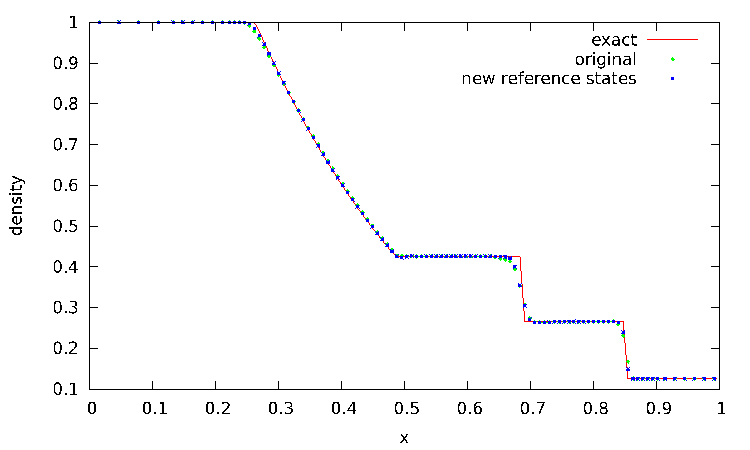
\includegraphics[scale=1.0]{reference}
  \caption{ \label{Fig:sod} Solution to Sod's problem with the original
    reference state and the new reference state, as compared to the
    exact solution.  We note that the new reference state shows a
    slightly sharper shock and contact, but also has a dip at the tail
    of the rarefaction.}
\end{figure}

\clearpage

%\begin{figure}
%  \centering
%  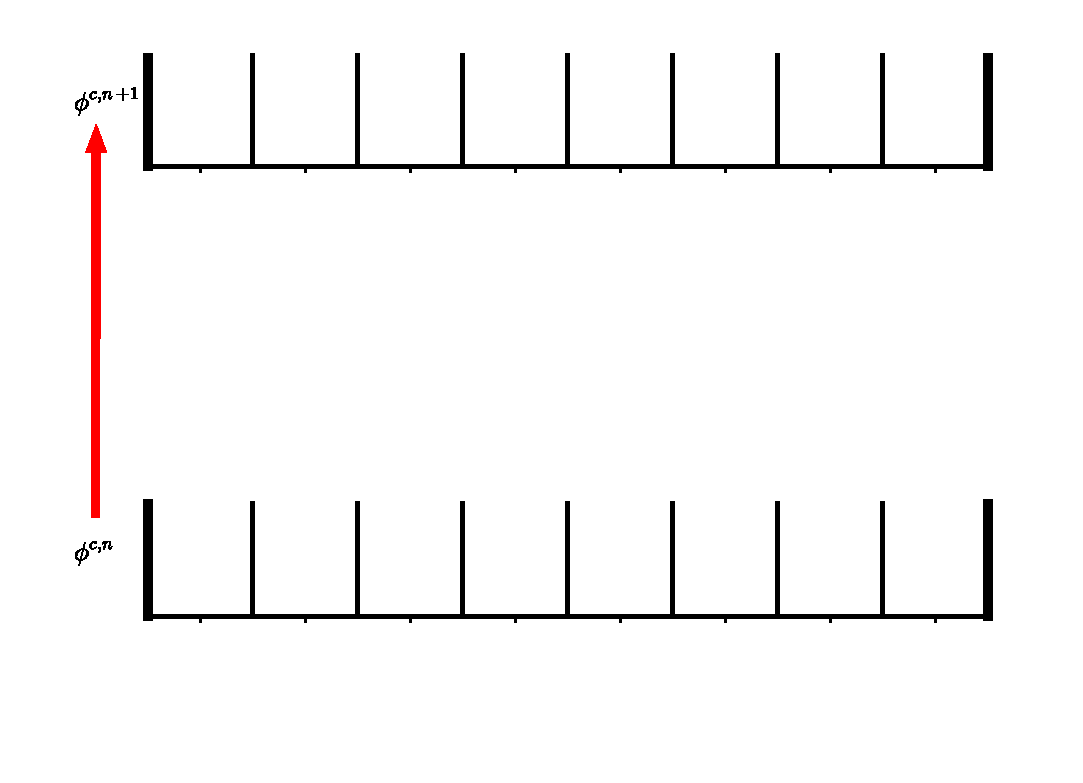
\includegraphics[width=3.1in]{nested2}\hspace{1em}
%  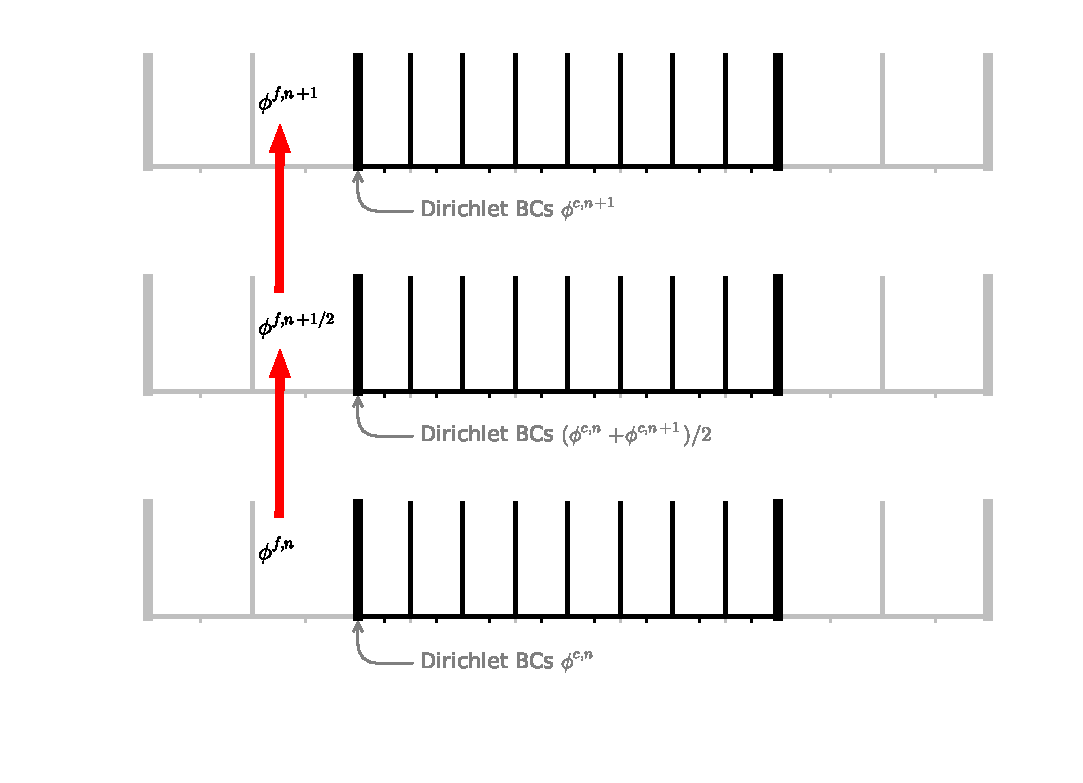
\includegraphics[width=3.1in]{nested3}
%  \caption{\label{fig:2levgrav} Schematic showing the solve for $\phi$ for a 2-level grid.}
%\end{figure}

\clearpage

\begin{figure}
  \centering
  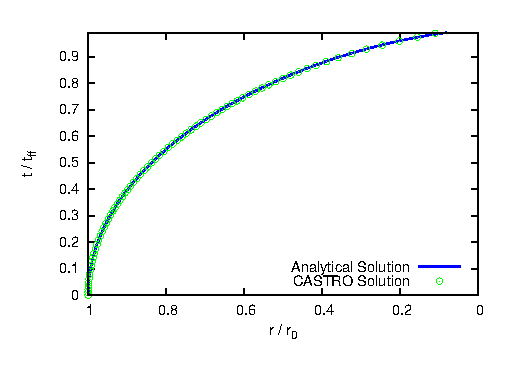
\includegraphics[scale=2.0]{freefall/plot_freefall}
  \caption{Time evolution of two initially stationary white dwarfs,
    mutually attracted to each other by the gravitational force. The
    horizontal axis gives the separation of the white dwarfs, scaled
    to the initial separation, and the vertical axis gives the elapsed
    time of the simulation, scaled to the total elapsed time
    necessarily. The solid curve shows the analytical result,
    calculated from Newtonian mechanics, and the circles show the
    samples from the time evolution with CASTRO. The agreement between
    theory and simulation is excellent, even for a simulation with
    modest resolution.}
  \label{Fig:Free Fall}
\end{figure}


\end{document}

